\usetikzlibrary{shapes.geometric}
\newcommand{\twoToneCircle}[4]{% #1: color of circle, 
                           % #2: color of semicircle
                           % #3: angle of semicircle 
                           % #4: center of semicircle 
 	\def\r{12pt}
    \node (s1) [circle,thick,draw=black, fill=#1, minimum size=\r, at={#4}] {};
    \node      [semicircle, fill=#2, 
                inner sep=0pt, outer sep=0pt, minimum size=\r/2+3,
                anchor=south, at={(s1.center)}, rotate=#3] {};
   }
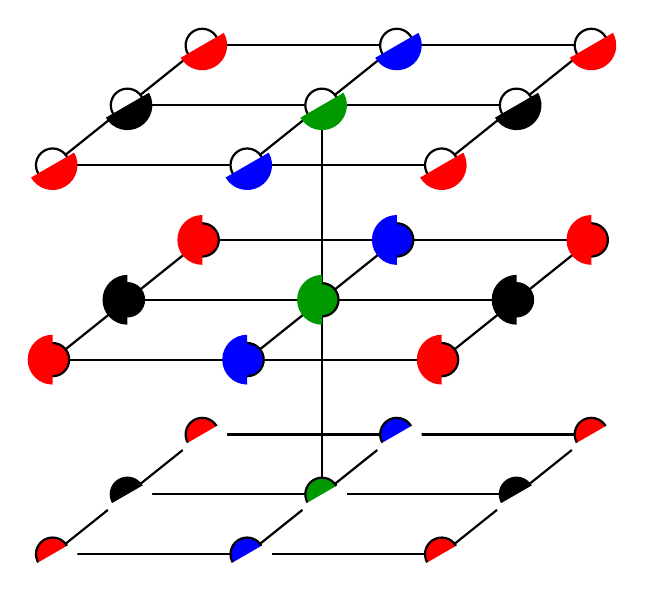
\begin{tikzpicture}[xscale=1.9,yscale=1.9]


\def\angle{90};
\def\angletop{210};
\def\anglebottom{\angletop}
\def\corner{red}
\def\bedge{black}
\def\cedge{blue}
\def\center{black!40!green}
\def\myfill{white}


\def\length{1.3};\def\offsetx{.5};\def\offsety{.4};\def\vertoffset{-1.3};


\coordinate (top_1) at (0,0);
\coordinate (top_2) at (\length,0);
\coordinate (top_3) at (2*\length,0);
\coordinate (top_4) at (\offsetx,\offsety);
\coordinate (top_5) at (\length+\offsetx,\offsety);
\coordinate (top_6) at (2*\length+\offsetx,\offsety);
\coordinate (top_7) at (2*\offsetx,2*\offsety);
\coordinate (top_8) at (\length+2*\offsetx,2*\offsety);
\coordinate (top_9) at (2*\length+2*\offsetx,2*\offsety);

\coordinate (mid_1) at (0,\vertoffset);
\coordinate (mid_2) at (\length,\vertoffset);
\coordinate (mid_3) at (2*\length,\vertoffset);
\coordinate (mid_4) at (\offsetx,\offsety+\vertoffset);
\coordinate (mid_5) at (\length+\offsetx,\offsety+\vertoffset);
\coordinate (mid_6) at (2*\length+\offsetx,\offsety+\vertoffset);
\coordinate (mid_7) at (2*\offsetx,2*\offsety+\vertoffset);
\coordinate (mid_8) at (\length+2*\offsetx,2*\offsety+\vertoffset);
\coordinate (mid_9) at (2*\length+2*\offsetx,2*\offsety+\vertoffset);

\coordinate (bot_1) at (0,2*\vertoffset);
\coordinate (bot_2) at (\length,2*\vertoffset);
\coordinate (bot_3) at (2*\length,2*\vertoffset);
\coordinate (bot_4) at (\offsetx,\offsety+2*\vertoffset);
\coordinate (bot_5) at (\length+\offsetx,\offsety+2*\vertoffset);
\coordinate (bot_6) at (2*\length+\offsetx,\offsety+2*\vertoffset);
\coordinate (bot_7) at (2*\offsetx,2*\offsety+2*\vertoffset);
\coordinate (bot_8) at (\length+2*\offsetx,2*\offsety+2*\vertoffset);
\coordinate (bot_9) at (2*\length+2*\offsetx,2*\offsety+2*\vertoffset);


\draw[thick,-] (top_1)--(top_7);
\draw[thick,-] (top_2)--(top_8);
\draw[thick,-] (top_3)--(top_9);
\draw[thick,-] (top_1)--(top_3);
\draw[thick,-] (top_4)--(top_6);
\draw[thick,-] (top_7)--(top_9);

\draw[thick,-] (mid_1)--(mid_7);
\draw[thick,-] (mid_2)--(mid_8);
\draw[thick,-] (mid_3)--(mid_9);
\draw[thick,-] (mid_1)--(mid_3);
\draw[thick,-] (mid_4)--(mid_6);
\draw[thick,-] (mid_7)--(mid_9);

\draw[thick,-] (bot_1)--(bot_7);
\draw[thick,-] (bot_2)--(bot_8);
\draw[thick,-] (bot_3)--(bot_9);
\draw[thick,-] (bot_1)--(bot_3);
\draw[thick,-] (bot_4)--(bot_6);
\draw[thick,-] (bot_7)--(bot_9);


%\draw[dashed] (top_1)--(bot_1);
%\draw[dashed] (top_2)--(bot_2);
%\draw[dashed] (top_3)--(bot_3);
%\draw[dashed] (top_4)--(bot_4);
\draw[thick,-] (top_5)--(bot_5);
%\draw[dashed] (top_6)--(bot_6);
%\draw[dashed] (top_7)--(bot_7);
%\draw[dashed] (top_8)--(bot_8);
%\draw[dashed] (top_9)--(bot_9);



  \twoToneCircle{\myfill}{\corner}{\angletop}{(top_1)};
  \twoToneCircle{\myfill}{\cedge}{\angletop}{(top_2)};
  \twoToneCircle{\myfill}{\corner}{\angletop}{(top_3)};
  \twoToneCircle{\myfill}{\bedge}{\angletop}{(top_4)};
  \twoToneCircle{\myfill}{\center}{\angletop}{(top_5)};
  \twoToneCircle{\myfill}{\bedge}{\angletop}{(top_6)};
  \twoToneCircle{\myfill}{\corner}{\angletop}{(top_7)};
  \twoToneCircle{\myfill}{\cedge}{\angletop}{(top_8)};
  \twoToneCircle{\myfill}{\corner}{\angletop}{(top_9)};
  
  \twoToneCircle{\corner}{\corner}{\angle}{(mid_1)};
  \twoToneCircle{\cedge}{\cedge}{\angle}{(mid_2)};
  \twoToneCircle{\corner}{\corner}{\angle}{(mid_3)};
  \twoToneCircle{\bedge}{\bedge}{\angle}{(mid_4)};
  \twoToneCircle{\center}{\center}{\angle}{(mid_5)};
  \twoToneCircle{\bedge}{\bedge}{\angle}{(mid_6)};
  \twoToneCircle{\corner}{\corner}{\angle}{(mid_7)};
  \twoToneCircle{\cedge}{\cedge}{\angle}{(mid_8)};
  \twoToneCircle{\corner}{\corner}{\angle}{(mid_9)};

  \twoToneCircle{\corner}{\myfill}{\anglebottom}{(bot_1)};
  \twoToneCircle{\cedge}{\myfill}{\anglebottom}{(bot_2)};
  \twoToneCircle{\corner}{\myfill}{\anglebottom}{(bot_3)};
  \twoToneCircle{\bedge}{\myfill}{\anglebottom}{(bot_4)};
  \twoToneCircle{\center}{\myfill}{\anglebottom}{(bot_5)};
  \twoToneCircle{\bedge}{\myfill}{\anglebottom}{(bot_6)};
  \twoToneCircle{\corner}{\myfill}{\anglebottom}{(bot_7)};
  \twoToneCircle{\cedge}{\myfill}{\anglebottom}{(bot_8)};
  \twoToneCircle{\corner}{\myfill}{\anglebottom}{(bot_9)};
\end{tikzpicture}







